\documentclass[11pt, a4paper, twoside]{article}
\usepackage[utf8]{inputenc}
\usepackage{graphicx}
\usepackage{listings}

 
\begin{document}
\date{2019 October}
\title{CS-443 Machine Learning Project 1: J-D-S Team}
\author{
  Julie Camille Rosalie Giunta\\
  \texttt{274957}
  \and
  Samuel Chassot\\
  \texttt{270955}
  \and
  Daniel Filipe Nunes Silva\\
  \texttt{275197}
}

\maketitle
\clearpage

\section{Introduction}
The goal of this project is to apply machine learning
methods learned in class on a real dataset. We take a
strong interest in testing a lot of techniques and
comparing their results. This comparison encourage us to
tweak hyperparameters and check their effectiveness using
cross-validation.

We do not use least\_squaresi\_SGD because we consider
that it would provide us results really close to other
methods we already us. Finally, we assess the following
methods.

\begin{itemize}
  \item least\_squares
  \item least\_squares\_GD 
  \item ridge\_regression
  \item logistic\_regression
  \item reg\_logistic\_regression
\end{itemize}
 
\section{other section}
This is not our report.



\section{Regularized logistic regression}
We implement cross-validation to optimize the values of $\lambda$ and $\gamma$. 
$\lambda$ takes values $\{1,10,100,1000,10000\}$ and $\gamma$ takes values $\{10^{-6},10^{-7},10^{-8},10^{-9}\}$. 
Taking bigger values for $\gamma$ results in the loss taking value $nan$. 
You can see the test error plotted against $\lambda$ in \ref{fig:raw_reg_log_regr}, 
each line corresponds to a value of $\gamma$.

\begin{figure}[h!]
  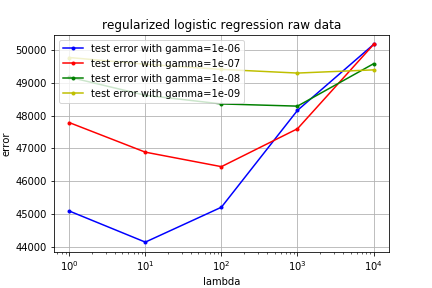
\includegraphics[width=\linewidth]{plots/raw_data_reg_log_regr.png}
  \caption{Regularized logistic regression - HP optimization}
  \label{fig:raw_reg_log_regr}
\end{figure}
\end{document}

\section{Least squares gradient descent}
To test the efficiency of \textit{least_squares_GD} on our dataset, which we standardize, we use cross-validation with five sets to train the hyperparameter $\gamma$.
In figure~\ref{fig:lsgd}, you can observe how fast the cross-validation test error is growing when you change gamma from $0.08$ to $0.09$ but in order to have a more useful representation of the progression of the error, you can take a look at figure~\ref{fig:lsgd_useful}, which omits the error corresponding to $\gamma = 0.09$.
For the initial weights chosen, they are first all initialized to $0.5$. We then modify the initial weights it to be closer to the final weights we got. Surprisingly, $0.4$ gives a better accuracy result on AICrowd ($69.7\%$) than $0.0$ ($69.3\%$) which is closer to the final weights in general and ouputs a smaller loss.
For the number of iterations, $200$ and $1000$ converge almost to the same loss so to be more efficient, we choose $200$.
Our best submission with \textit{least_squares_GD} has an accuracy of $69.7\%$ and has, as hyperparameters,
\begin{lstlisting}
max_iters = 200
k_fold = 5
initial_weights = np.array([0.4 for i in range(tX_stdrzed.shape[1])])
gamma = 0.08
\end{lstlisting}

\begin{figure}
    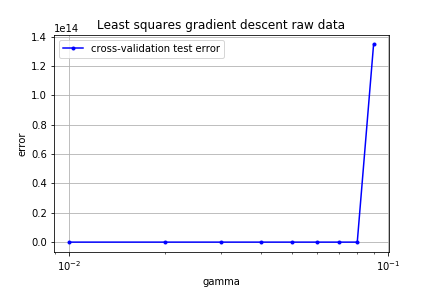
\includegraphics[width= 3, height = 3]{raw_data_least_squares_GD.png}
    \label{fig:lsgd}
\end{figure}

\begin{figure}
    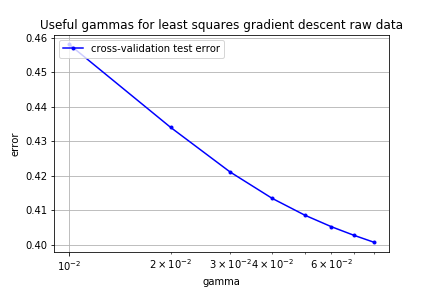
\includegraphics[width= 3, height = 3]{raw_data_least_squares_GD_useful.png}
    \label{fig:lsgd_useful}
\end{figure}

\section{Logistic regression}
We also used cross-validation to test the efficiency of \textit{logistic_regression} on our standardized dataset.
We use five sets to set the hyperparameter $\gamma$.
For the initial weights chosen, they are all initialized to $0.5$ since $0.0, 0.1, ..., 0.6$ do not change the loss a lot but worsen the accuracy on AICrowd.
Our best submission with \textit{logistic_regression} had an accuracy of $73.9\%$ and had 
\begin{lstlisting}
max_iters = 1000
k_fold = 5
initial_weights = np.array([0.5 for i in range(tX_stdrzed.shape[1])])
gamma = 1e-06
\end{lstlisting}

\begin{figure}
    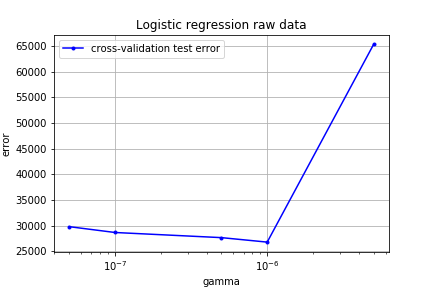
\includegraphics[width= 3, height = 3]{raw_data_logistic_regression.png}
    \label{fig:log_reg}
\end{figure}

\end{document}